\documentclass[12pt]{report}
\usepackage[spanish]{babel}
\usepackage[utf8]{inputenc}
\usepackage{graphicx}
\usepackage{verbatim}
\usepackage{listings}
\usepackage{float}
\renewcommand*\thesection{\arabic{section}}

\begin{document}
	
	\begin{center}
		\textbf{Análisis de Algoritmos, Sem: 2018-1, 3CV1, Práctica 3, 09-2017}
		\newline
	\end{center}
	
	\begin{center}
		\begin{picture}(0,0) \put(-125,-55){
			\includegraphics[width=2.7cm]{../../IPNlogo.jpg}} 
		\end{picture}
		\LARGE Escuela Superior de Cómputo.\\
		Instituto Politécnico Nacional, México.\\
		\begin{picture}(0,0) \put(160,10){
			\includegraphics[width=2.7cm]{../../logoescom.png}} 
		\end{picture}
	\end{center}
	
	\begin{center}
		\Large Práctica 3: Divide y Vencerás. Algoritmo MergeSort.\\
	\end{center}
	
	\begin{center}
		\textbf{Blancas Pérez Bryan Israel}\\
		orionmunecaycanica@gmail.com\\
	\end{center}
	
	
	\textbf{\large Resumen: }Aplicar la técnica "Divide y Vencerás", específicamente con el algoritmo de ordenamiento MergeSort, y encontrar el orden de complejidad de éste.\newline\\
	
	\textbf{\large Palabras Clave: } Divide y Vencerás, Merge, MergeSort.\\
	

	\section{Introducción}
		En ocasiones, existen problemas complicados de resolver si se abordan como uno solo, comúnmente a estos problemas se les aplica un enfoque de "Divide y Vencerás". En está práctica se muestra el empleo de esta técnica para ordenar arreglos de números, utilizando el algoritmo MergeSort.\newpage
	

	\section{Conceptos Básicos}
	\textbf{Divide y Vencerás.}\\
		
		El enfoque "Divide y Vencerás", está basado en la resolución recursiva de un problema, separándolo en sub-problemas hasta que éstos lleguen  a ser suficientemente sencillos para resolverlos directamente, para luego combinar las soluciones de esos sub-problemas para resolver el problema principal [1]. Se puede explicar el método en tres pasos. \newline \newline
		1. \textbf{Divide} el problema en sub-problemas de la misma naturaleza.\newline
		2. \textbf{Vence} a los sub-problemas sencillos resolviéndolos.\newline
		3. \textbf{Combina} las soluciones de los sub-problemas para resolver el problema principal.\\
		
	\textbf{MergeSort.}\\
	
	MergeSort es un algoritmo de ordenamiento basado en la técnica "Divide y Vencerás". Fue desarrollado por John Von Neumann 1945. [2]\\
	Este algoritmo divide una la lista desordenada hasta que quedan sublistas de tamaño uno, las cuales, por concepto, ya están ordenadas. Una vez hecho esto, utiliza el algoritmo Merge para comparar y ordenar las sublistas, para luego mezclarlas en una sola lista, así sucesivamente hasta ordenar todo el arreglo original.
	
	\section{Experimentación y Resultados}	
	\textbf{Ejercicio 1.}\\
	Implementar el algoritmo MergeSort.\newline \newline
	Pseudocódigo del algoritmo Merge:
	\lstset{language=C, breaklines=true, basicstyle=\footnotesize}
	\lstset{numbers=left, numberstyle=\tiny, stepnumber=1, numbersep=10pt}
	\begin{lstlisting}
Merge(A,p,q,r)
  n1=q-p+1
  n2=r-q
  
  Sean L[0,...,n1-1] y R[0,...,n2-1]
  
  
  for i=0 to i < n1 do
    L[i]=A[p+i]
  for j=0 to j < n2 do
    R[j]=A[q+1+j]
   
  i=j=0
  
  for k = p to k <= r do
    if L[i] <= R[j]
      A[k] = L[i]
      i++
    else 
      A[k] = R[j]
      j++
      
	\end{lstlisting}
	
	El algoritmo Merge, recibe como entrada un arreglo $A[p,..,q,...,r]$ bajo la premisa de que los números de $p$ a $q$ están ordenados de manera creciente, al igual que los números de $q+1$ a $r$. Como salida, el algoritmo devuelve el arreglo $A[p,..,q,...,r]$ ordenado de manera creciente. \\

	Pseudocódigo del algoritmo MergeSort:
	\lstset{language=C, breaklines=true, basicstyle=\footnotesize}
	\lstset{numbers=left, numberstyle=\tiny, stepnumber=1, numbersep=10pt}
	\begin{lstlisting}
MergeSort(A[p,...r],p,r)
  if p < r then
    q = (p+r)/2
    MergeSort(A[p,...,r],p,q)
    MergeSort(A[p,...,r],q+1,r)
    Merge(A,p,q,r)
	\end{lstlisting}
	
	El algoritmo MergeSort, recibe como entrada un arreglo $A[p,...,r]$, arreglo que va dividiendo por medio de llamadas recursivas. Se realiza esa operación hasta que p = r, es decir, cuando se halla dividido el arreglo A en subarreglos de tamaño uno. Una vez hecho esto, se hace uso de la función Merge, la cual ordenará esos subarreglos en orden creciente. MergeSort devuelve al arreglo A ordenado de crecientemente.\newpage
	
	
	\textbf{Ejecución de la función Merge\\}
	\begin{figure}[H]
		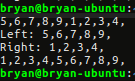
\includegraphics[width=4cm]{imagenes/1.png}
		\centering
		\caption{Ejecución del algoritmo Merge.}
		\centering
	\end{figure}
	En la figura 1, se aprecia la ejecución del algoritmo Merge. Como se puede ver, recibe un arreglo el cual tiene las mitades ordenadas crecientemente. Se muestra parte del procedimiento, imprimiendo cómo el algoritmo ha separado el arreglo original en dos subarreglos. Como salida se muestra todo el arreglo ordenado de manera creciente.\\
	
	Gráfica del orden de complejidad del algoritmo Merge.\\
	\begin{figure}[H]
		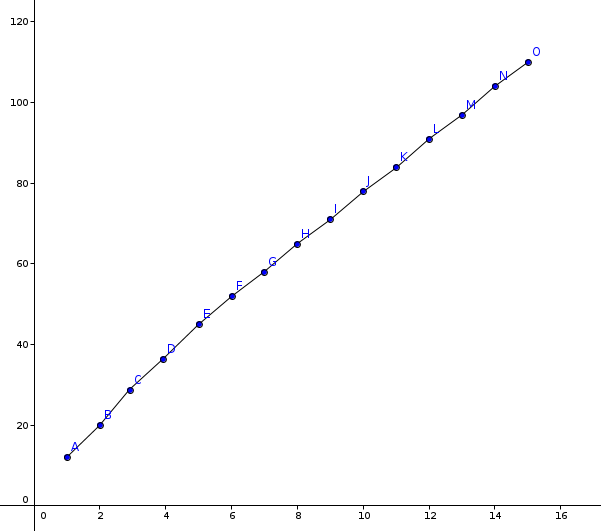
\includegraphics[height=5cm]{imagenes/output1_grafica.png}
		\centering
		\caption{Gráfica del orden de complejidad del algoritmo Merge.}
		\centering
	\end{figure}
	En la figura 2, se muestra la gráfica $T(n) \ vs \ n$. Como es apreciable, el orden de complejidad del algoritmo Merge, para ordenar un arreglo tiene orden de complejidad lineal. Observación: la gráfica muestra "saltos" debido a las condiciones implementadas en el algoritmo para su correcto funcionamiento, las cuales modifican $T(n)$ (cont). \newpage
	
	Demostración analítica del orden de complejidad del algoritmo Merge.\\
	
\lstset{language=C, breaklines=true, basicstyle=\footnotesize}
\lstset{numbers=left, numberstyle=\tiny, stepnumber=1, numbersep=10pt}
\begin{lstlisting}
Merge(A,p,q,r)
  n1=q-p+1
  n2=r-q
  Sean L[0,...,n1-1] y R[0,...,n2-1]

  for i=0 to i < n1 do
    L[i]=A[p+i]
  for j=0 to j < n2 do
    R[j]=A[q+1+j]

  i=j=0

  for k = p to k <= r do
    if L[i] <= R[j]
      A[k] = L[i]
      i++
    else 
      A[k] = R[j]
      j++

\end{lstlisting}

\begin{table}[htbp]
	\begin{center}
		\begin{tabular}{|l|l|}
			\hline
			\multicolumn{2}{|c|}{Análisis del Algoritmo} \\ 
			\hline
			\textbf{Línea de Código} & \textbf{Orden de complejidad}\\
			\hline
			2 & $\theta (1)$ \\ \hline
			3 & $\theta (1)$ \\ \hline
			4 & $\theta (1)$ \\ \hline
			6 & $\theta (n1)$ \\ \hline
			8 & $\theta (n2)$ \\ \hline
			11 & $\theta (1)$ \\ \hline
			13 & $\theta (r-p+1)= \theta (n)$ \\ \hline
		\end{tabular}
		\caption{Análisis del algoritmo.}
		\label{tabla:analisis1}
	\end{center}
\end{table}
Aclaración: como las lineas de código dentro de los $for's$ son orden $\theta (1)$, por el teorema de la multiplicación $t_{1}(n)t_{2}(n) \ \epsilon \ \theta (f_{1}(n)f_{2}(n)$, consideramos unicamente el orden de complejidad de la linea del $for$.\newpage
Entonces.\\
$T(n)=\theta (1) + \theta (1) + \theta (1) +\theta (n1) + \theta (n2) + \theta (1) + \theta (n).$\\
Pero\\
$\theta (n1) + \theta (n2) = \theta (n).$ Puesto que $n$ fue particionado en $n1$ y $n2$.\\
Entonces.\\
$T(n)=\theta (1) + \theta (1) + \theta (1) +\theta (n) + \theta (1) + \theta (n).$\\
Y por el teorema de la suma $t_{1}(n)+t_{2}(n) \ \epsilon \ \theta (max(f_{1}(n),f_{2}(n))$.
Entonces.
$T(n)=\theta (n).$\\

$Por \ lo \ tanto \ , \ T(n) \epsilon \ \theta (n)$\\


\textbf{Ejecución de la función MergeSort\\}
\begin{figure}[H]
	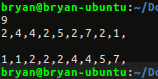
\includegraphics[width=4cm]{imagenes/2.png}
	\centering
	\caption{Ejecución del algoritmo MergeSort.}
	\centering
\end{figure}
En la figura 3, se aprecia la ejecución del algoritmo MergeSort. Como se puede ver, recibe como entrada un número n, el cual representa el largo del arreglo a ordenar. Una vez introducido el número, se crea el arreglo tamaño n y se llena con números aleatorios. Como salida, MergeSort devuelve el arreglo ordenado de manera creciente.\newpage

Gráfica del orden de complejidad del algoritmo MergeSort.\\
\begin{figure}[H]
	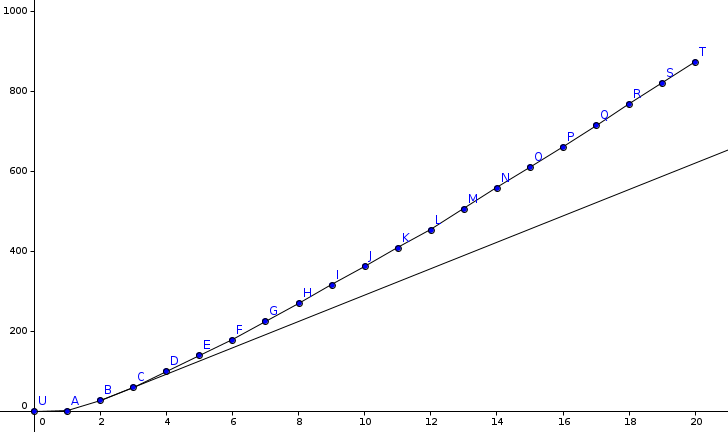
\includegraphics[height=5cm]{imagenes/output2_grafica.png}
	\centering
	\caption{Gráfica del orden de complejidad del algoritmo MergeSort.}
	\centering
\end{figure}
En la figura 4, se muestra la gráfica $T(n) \ vs \ n$. En la gráfica, la curva se aprecia muy poco si se deja sola, así que de manera auxiliar para probar que existe esa curvatura, trace una recta que pasa por los puntos B y C.
Como se puede ver, el orden de complejidad del algoritmo MergeSort es nlogn.\\

Demostración analítica del orden de complejidad del algoritmo MergeSort.\\

\lstset{language=C, breaklines=true, basicstyle=\footnotesize}
\lstset{numbers=left, numberstyle=\tiny, stepnumber=1, numbersep=10pt}
\begin{lstlisting}
MergeSort(A[p,...r],p,r)
  if p < r then
    q = (p+r)/2
    MergeSort(A[p,...,r],p,q)
    MergeSort(A[p,...,r],q+1,r)
    Merge(A,p,q,r)

\end{lstlisting}
\newpage
\begin{table}[htbp]
	\begin{center}
		\begin{tabular}{|l|l|}
			\hline
			\multicolumn{2}{|c|}{Análisis del Algoritmo} \\ 
			\hline
			\textbf{Línea de Código} & \textbf{Orden de complejidad}\\
			\hline
			3 & $\theta (1)$ \\ \hline
			4 & $T(n/2)$ \\ \hline
			5 & $T(n/2)$ \\ \hline
			6 & $Cn$ (previamente demostrado) \\ \hline
		\end{tabular}
		\caption{Análisis del algoritmo.}
		\label{tabla:analisis2}
	\end{center}
\end{table}

Entonces.\\
 $T(n) = \left \{ \begin{array}{c} \theta (1) \ si \ n=1 \\ 2T(n/2)+Cn \ si \ n \ > \ 1 \end{array}\right.$\\
 pero $\theta (1)= C$, entonces\\
  $T(n) = \left \{ \begin{array}{c} C \ si \ n=1 \\ 2T(n/2)+Cn \ si \ n \ > \ 1 \end{array}\right.$\\
  Así tenemos: \\
  
  Sea $n | k=log_{2}(n)$, \\
   $T(2^{k}) = \left \{ \begin{array}{c} C \ si \ 2^{k}=1 \\ 2T(2^{k-1})+C2^{k} \ si \ 2^{k} \ > \ 1 \end{array}\right.$\\
Usando el método de sustitución hacia atrás.\\
$T(2^{k})=2^{2}T(2^{k-2})+2C2^{k}$\\
$T(2^{k})=2^{3}T(2^{k-3})+3C2^{k}$\\
$T(2^{k})=2^{i}T(2^{k-i})+iC2^{k}$\\
cuando i=k\\
$T(2^{k})=2^{k}T(2^{k-k})+kC2^{k}$\\
$T(2^{k})=2^{2}T(1)+kC2^{k}$\\
$T(2^{k})=C2^{k}+kC2^{k}$\\
$T(2^{k})=(k+1)C2^{k}$\\
pero $k=log_{2}(n)$, entonces
$T(2^{k})=(log_{2}(n)+1)Cn$\\
$T(2^{k})=Cnlog_{2}(n)+Cn$\\

$Por \ lo \ tanto \ , \ T(n) \epsilon \ \theta (nlog_{2}(n))$


	
\section{Conclusiones}
Esta práctica me pareció muy buena para entender el concepto de "Divide y Vencerás", y aparte de comprenderlo, lo pudimos aplicar al hacer el algoritmo MergeSort. Tuve un par de complicaciones al hacer el algoritmo Merge, ya que al principio no tenia bien claro que, para que funcione el algoritmo, es necesario que el algoritmo este dividido en dos arreglos \textbf{ya} ordenados previamente. Como yo no estaba tomando en cuenta eso, el algoritmo no funcionaba.\\ La otra complicación que tuve, fue al darme cuenta de que, al momento de comparar los subarreglos, existen casos en los que los índices se acaban, pero lo solucioné poniendo un par de condiciones para ordenar el resto del arreglo.\\
Los resultados fueron los esperados, y a mi parecer esta fue una práctica muy productiva, tanto teórica como prácticamente.\newpage 
	

\section{Anexo}
	
Calcular el orden de complejidad de los siguientes algoritmos en el mejor ($\Omega$) y en el peor de los casos (O) (no es necesario hacer el análisis línea por línea, en este caso, pueden aplicar propiedades de los algoritmos vistos en clase):\\

	\textbf{A.}
	\lstset{language=vhdl, breaklines=true, basicstyle=\footnotesize}
	\lstset{numbers=left, numberstyle=\tiny, stepnumber=1, numbersep=10pt}
	\begin{lstlisting}
Funcion1(n par)
  i=0
  mientras i < n hacer
    para j = 1 hasta j = 10 hacer
      accion(i)
      j++
    i+=2
	\end{lstlisting}
	Suponga Accion(i) $\epsilon \ \theta (1).$\\
	
	\begin{table}[htbp]
		\begin{center}
			\begin{tabular}{|l|l|}
				\hline
				\multicolumn{2}{|c|}{Análisis del Algoritmo} \\ 
				\hline
				\textbf{Línea de Código} & \textbf{Orden de complejidad}\\
				\hline
				2 & $\theta (1)$ \\ \hline
				3 & $\theta (n/2)$ \\ \hline
				4 & $\theta (1)$ \\ \hline
				5 & $\theta (1)$ \\ \hline
				6 & $\theta (1)$ \\ \hline
				7 & $\theta (1)$ \\ \hline
			\end{tabular}
			\caption{Análisis del algoritmo.}
			\label{tabla:analisis3}
		\end{center}
	\end{table}
	
	Entonces el código dentro del $while$ tiene orden de complejidad constante, por lo tanto el bloque $while$, aplicando el teorema de la multiplicación, queda con orden $\theta (n)$.\\
	El bloque $while$ depende de $n$, sin hacer distinción entre el peor y mejor caso.\\
	
	$Por \ lo \ tanto \ Funcion1 \ \epsilon \ \theta (n)$.\newpage
		
	\textbf{B.}
	\lstset{language=vhdl, breaklines=true, basicstyle=\footnotesize}
	\lstset{numbers=left, numberstyle=\tiny, stepnumber=1, numbersep=10pt}
	\begin{lstlisting}
Funcion2(A[0,...,n-1, x entero])
  for i = 0 to i < n do
    if A[i] < x then
      A[i]=min(A[0,...,n-1])
    else if A[i] > x then
      A[i]=max(A[0,...,n-1])
    else
      exit
	\end{lstlisting}
	
	\begin{table}[htbp]
		\begin{center}
			\begin{tabular}{|l|l|}
				\hline
				\multicolumn{2}{|c|}{Análisis del Algoritmo} \\ 
				\hline
				\textbf{Línea de Código} & \textbf{Orden de complejidad}\\
				\hline
				2 & $\theta (n)$ \\ \hline
				3 & $\theta (1)$ \\ \hline
				4 & $\theta (n)$ \\ \hline
				5 & $\theta (1)$ \\ \hline
				6 & $\theta (n)$ \\ \hline
				7 & $\theta (1)$ \\ \hline
				8 & $\theta (1)$ \\ \hline
			\end{tabular}
			\caption{Análisis del algoritmo.}
			\label{tabla:analisis4}
		\end{center}
	\end{table}
	
	El min y max de un arreglo tiene orden de complejidad n debido a que es necesario recorrer todo el arreglo para encontrar el número que cumpla a condición. 
	
	Entonces. \\
	
	Si $A[i]=x \ , \ i=0,1,2,...,n-1.$\\
	
	Entonces $Funcion2 \ \epsilon \ \Omega(n)$, debido a que las líneas de código 4 y 6 jamás se ejecutan por que la condición en la que están se los impide.\\
	
	Y si $A[i]\neq x \ , \ i=0,1,2,...,n-1.$\\
	
	Entonces $Funcion2 \ \epsilon \ O(n^{2})$, debido a que las líneas de código 4 y 6 se pueden ejecutar, y por el teorema de la multiplicación, los se multiplican. 
	
	\section{Bibliografía}
	
	[1] https://es.wikipedia.org/wiki/Algoritmo\_divide\_y\_vencerás\\
	
	[2] https://en.wikipedia.org/wiki/Merge\_sort
\end{document}